%
% ---------------------------------------------------------------
% Copyright (C) 2012-2018 Gang Li
% ---------------------------------------------------------------
%
% This work is the default powerdot-tuliplab style test file and may be
% distributed and/or modified under the conditions of the LaTeX Project Public
% License, either version 1.3 of this license or (at your option) any later
% version. The latest version of this license is in
% http://www.latex-project.org/lppl.txt and version 1.3 or later is part of all
% distributions of LaTeX version 2003/12/01 or later.
%
% This work has the LPPL maintenance status "maintained".
%
% This Current Maintainer of this work is Gang Li.
%
%

\documentclass[
 size=14pt,
 paper=smartboard,  %a4paper, smartboard, screen
 mode=present, 		%present, handout, print
 display=slides, 	% slidesnotes, notes, slides
 style=tuliplab,  	% TULIP Lab style
 pauseslide,
 fleqn,leqno]{powerdot}


\usepackage{cancel}
\usepackage{caption}
\usepackage{stackengine}
\usepackage{smartdiagram}
\usepackage{attrib}
\usepackage{amssymb}
\usepackage{amsmath} 
\usepackage{amsthm} 
\usepackage{mathtools}
\usepackage{rotating}
\usepackage{graphicx}
\usepackage{boxedminipage}
\usepackage{rotate}
\usepackage{calc}
\usepackage[absolute]{textpos}
\usepackage{psfrag,overpic}
\usepackage{fouriernc}
\usepackage{pstricks,pst-3d,pst-grad,pstricks-add,pst-text,pst-node,pst-tree}
\usepackage{moreverb,epsfig,subfigure}
\usepackage{color}
\usepackage{booktabs}
\usepackage{etex}
\usepackage{breqn}
\usepackage{multirow}
\usepackage{natbib}
\usepackage{bibentry}
\usepackage{gitinfo2}
\usepackage{siunitx}
\usepackage{nicefrac}
%\usepackage{geometry}
%\geometry{verbose,letterpaper}
\usepackage{media9}
\usepackage{animate}
%\usepackage{movie15}
\usepackage{auto-pst-pdf}

\usepackage{breakurl}
\usepackage{fontawesome}
\usepackage{xcolor}
\usepackage{multicol}


\usepackage{mdwlist} 
\usepackage{verbatim}
\usepackage[utf8]{inputenc}
\usepackage{dtk-logos}
\usepackage{tikz}
\usepackage{adigraph}
%\usepackage{tkz-graph}
\usepackage{hyperref}
%\usepackage{ulem}
\usepackage{pgfplots}
\usepackage{verbatim}
\usepackage{fontawesome}


\usepackage{todonotes}
% \usepackage{pst-rel-points}
\usepackage{animate}
\usepackage{fontawesome}
\usepackage{makecell}
\usepackage{listings}
\lstset{frameround=fttt,
frame=trBL,
stringstyle=\ttfamily,
backgroundcolor=\color{yellow!20},
basicstyle=\footnotesize\ttfamily}
\lstnewenvironment{code}{
\lstset{frame=single,escapeinside=`',
backgroundcolor=\color{yellow!20},
basicstyle=\footnotesize\ttfamily}
}{}


\usepackage{hyperref}
\hypersetup{ % TODO: PDF meta Data
  pdftitle={Presentation Title},
  pdfauthor={Gang Li},
  pdfpagemode={FullScreen},
  pdfborder={0 0 0}
}


% \usepackage{auto-pst-pdf}
% package to show source code

\definecolor{LightGray}{rgb}{0.9,0.9,0.9}
\newlength{\pixel}\setlength\pixel{0.000714285714\slidewidth}
\setlength{\TPHorizModule}{\slidewidth}
\setlength{\TPVertModule}{\slideheight}
\newcommand\highlight[1]{\fbox{#1}}
\newcommand\icite[1]{{\footnotesize [#1]}}

\newcommand\twotonebox[2]{\fcolorbox{pdcolor2}{pdcolor2}
{#1\vphantom{#2}}\fcolorbox{pdcolor2}{white}{#2\vphantom{#1}}}
\newcommand\twotoneboxo[2]{\fcolorbox{pdcolor2}{pdcolor2}
{#1}\fcolorbox{pdcolor2}{white}{#2}}
\newcommand\vpspace[1]{\vphantom{\vspace{#1}}}
\newcommand\hpspace[1]{\hphantom{\hspace{#1}}}
\newcommand\COMMENT[1]{}

\newcommand\placepos[3]{\hbox to\z@{\kern#1
        \raisebox{-#2}[\z@][\z@]{#3}\hss}\ignorespaces}

\renewcommand{\baselinestretch}{1.2}


\newcommand{\draftnote}[3]{
	\todo[author=#2,color=#1!30,size=\footnotesize]{\textsf{#3}}	}
% TODO: add yourself here:
%
\newcommand{\gangli}[1]{\draftnote{blue}{GLi:}{#1}}
\newcommand{\shaoni}[1]{\draftnote{green}{sn:}{#1}}
\newcommand{\gliMarker}
	{\todo[author=GLi,size=\tiny,inline,color=blue!40]
	{Gang Li has worked up to here.}}
\newcommand{\snMarker}
	{\todo[author=Sn,size=\tiny,inline,color=green!40]
	{Shaoni has worked up to here.}}

%%%%%%%%%%%%%%%%%%%%%%%%%%%%%%%%%%%%%%%%%%%%%%%%%%%%%%%%%%%%%%%%%%%%%%%%
% title
% TODO: Customize to your Own Title, Name, Address
%
\title{Traffic Flow Prediction In a U.S. Metropolis}
\author{
Jingbao Luo
\\
\\Nanjing University of Science and Technology
\\Deakin University
}
\date{\gitCommitterDate}


% Customize the setting of slides
\pdsetup{
% TODO: Customize the left footer, and right footer
rf=\href{http://www.tulip.org.au}{
Last Changed by: \textsc{\gitCommitterName}\ \gitVtagn -\gitAbbrevHash\ (\gitAuthorDate)
},
cf={Traffic Flow Prediction In a U.S Metropolis},
}


\begin{document}

\maketitle

%\begin{slide}{Overview}
%\tableofcontents[content=sections]
%\end{slide}


%%==========================================================================================
%%
\begin{slide}[toc=,bm=]{Overview}
\tableofcontents[content=currentsection,type=1]
\end{slide}
%%
%%==========================================================================================


\section{Problem Definition}


%%==========================================================================================
%%
\begin{slide}{Tabular Playground Series - Mar 2022}
\begin{center}

\twotonebox{\rotatebox{90}{Defn}}{\parbox{.86\textwidth}
{The March edition of the 2022 Tabular Playground Series
 is a prediction project about time series data.
\begin{itemize}
\item We'll forecast twelve-hours of traffic flow in a major U.S. metropolitan area. 
Time, space, and directional features give us the chance to model interactions across a network of roadways.
\end{itemize}
}}
\end{center}
\begin{table}[htbp]
	\setlength{\abovecaptionskip}{0pt}
	\setlength{\belowcaptionskip}{10pt}
	\centering
	\caption{DATA}
\begin{tabular}{ c | c | c }
	\toprule
	% after \\: \hline or \cline{col1-col2} \cline{col3-col4} ...
	File    &Description      & Attribution       \\
	\midrule
	train.csv       &  \makecell{traffic congestion from April\\through September of 1991}   &  \makecell{row_id,time,x,y,\\direction,congestion}       \\
	\midrule
	test.csv       & \makecell{hourly predictions \\on the day of 1991-09-30}   &\makecell{row_id,time,x,y,\\direction}     \\
	\bottomrule
\end{tabular}
\end{table}

\end{slide}
%%
%%==========================================================================================
\section{Data Processing}
%%==========================================================================================
%%
\begin{slide}{Data Processing}
\begin{itemize}
\item
Split time data
\item
Merge x,y,direction data

\vspace{1cm}
\twocolumn[
\savevalue{lfrheight}=8.5cm,
\savevalue{lfrprop}={
linestyle=solid,framearc=.2,linewidth=1pt},
rfrheight=\usevalue{lfrheight},
rfrprop=\usevalue{lfrprop}
]{
\setlength{\leftskip}{10pt}
Data split and merge
\begin{itemize}
\setlength{\itemsep}{-0.9ex} 
\item
\smallskip  
month
\item
\smallskip
weekday
\item
\smallskip
minute
\item
\smallskip
is_month_start
\item
\smallskip
is_month_end
\item
\smallskip
is_weekday
\item
\smallskip
is_Monday
\item
\smallskip
is_Friday
\item
\smallskip
period
\item
\smallskip
road:x+y+direction(00EB)
\end{itemize}
}
{
\setlength{\leftskip}{10pt}
Period
\begin{itemize}
\item
\smallskip
Late Night: 0:00-4:00
\item
\smallskip
Early Morning: 4:00-8:00
\item
\smallskip
Morning: 8:00-12:00
\item
\smallskip
Noon: 12:00-16:00
\item
\smallskip
Evening: 16:00-20:00
\item
\smallskip
Night: 20:00-24:00
\end{itemize}
}
\end{itemize}



\end{slide}
%%
%%==========================================================================================
\section{Data Description}

%%==========================================================================================
%%
\begin{slide}[toc=,bm=]{Train data decription}
\vspace{1.2cm}
\begin{figure}
	\setlength{\abovecaptionskip}{0.5cm}
    \centering
    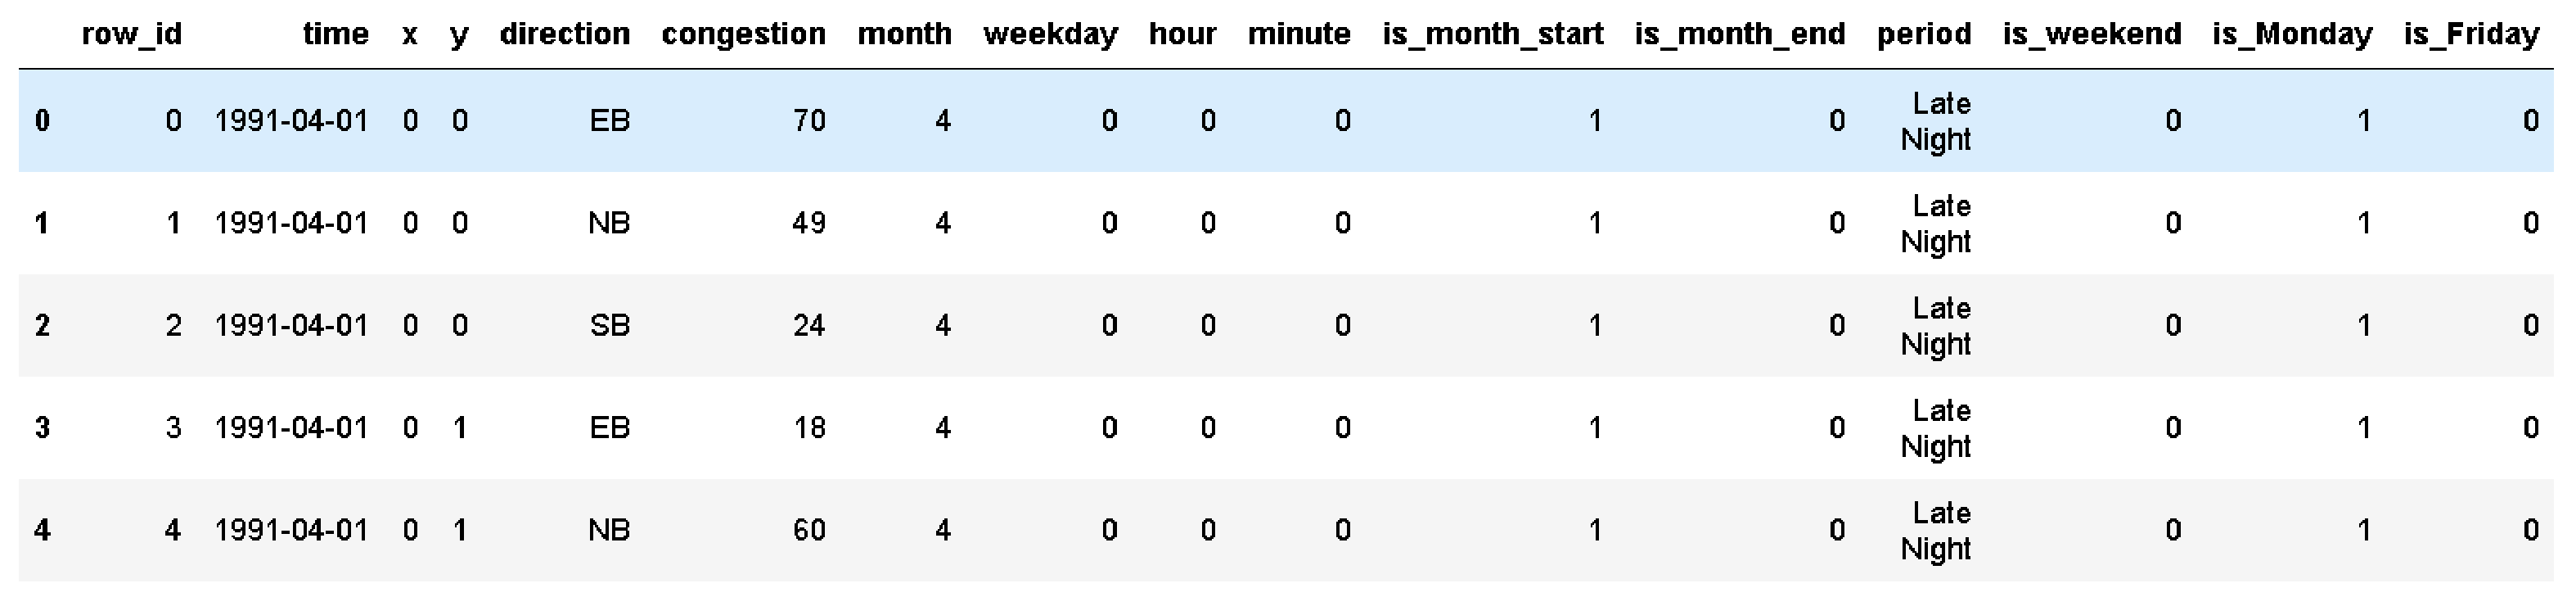
\includegraphics[scale=0.38]{figure/train_data.eps}\\	
    \caption{train_data}
    \label{fig:train_data}
\end{figure}
\end{slide}
%%
%%==========================================================================================
\begin{slide}[toc=,bm=]{Congestion data}
\begin{figure}
	\setlength{\abovecaptionskip}{-0.2cm} %调整图片标题与图距离
	\includegraphics[scale=0.9]{figure/congestion.eps}\\	
	\caption{Congestion data}
	\label{Congestion data}
\end{figure}
\end{slide}
%%
%%==========================================================================================
\begin{slide}[toc=,bm=]{The effect of weekday on congestion}
	\begin{figure}
		\setlength{\abovecaptionskip}{-0.2cm} %调整图片标题与图距离
		\includegraphics[scale=0.9]{figure/weekday.eps}\\	
		\caption{The effect of weekday on congestion}
		\label{weekday}
	\end{figure}
\end{slide}
%%
%%==========================================================================================
\begin{slide}[toc=,bm=]{Congestion in special day or not}
	\begin{figure}
		\setlength{\abovecaptionskip}{0.2cm} 
		\raggedleft
		\includegraphics[scale=0.65]{figure/is_weekend.eps}
		\centering
		\caption{Congestion in special day or not}
		\label{special}
	\end{figure}
\end{slide}
%%
%%==========================================================================================
\begin{slide}[toc=,bm=]{The effect of road on congestion }
	\begin{center}
		\begin{figure}
			\setlength{\abovecaptionskip}{0.4cm} 
			\raggedleft
			\includegraphics[scale=0.32]{figure/road1.eps}
			\centering
			\caption{The effect of road on congestion}
			\label{road}
		\end{figure}
	\end{center}
	\end{slide}
%%
%%==========================================================================================
\begin{slide}[toc=,bm=]{The effect of day on congestion group by month }
\begin{center}
	\begin{figure}
		\setlength{\abovecaptionskip}{0.5cm} 
		\raggedleft
		\includegraphics[scale=0.4]{figure/day.eps}
		\centering
		\caption{The effect of day on congestion group by month}
		\label{day}
	\end{figure}
\end{center}
\end{slide}
%%
%%==========================================================================================
\begin{slide}[toc=,bm=]{The effect of hour on congestion group by road }
	\begin{figure}
		\setlength{\abovecaptionskip}{0.4cm} 
		\raggedleft
		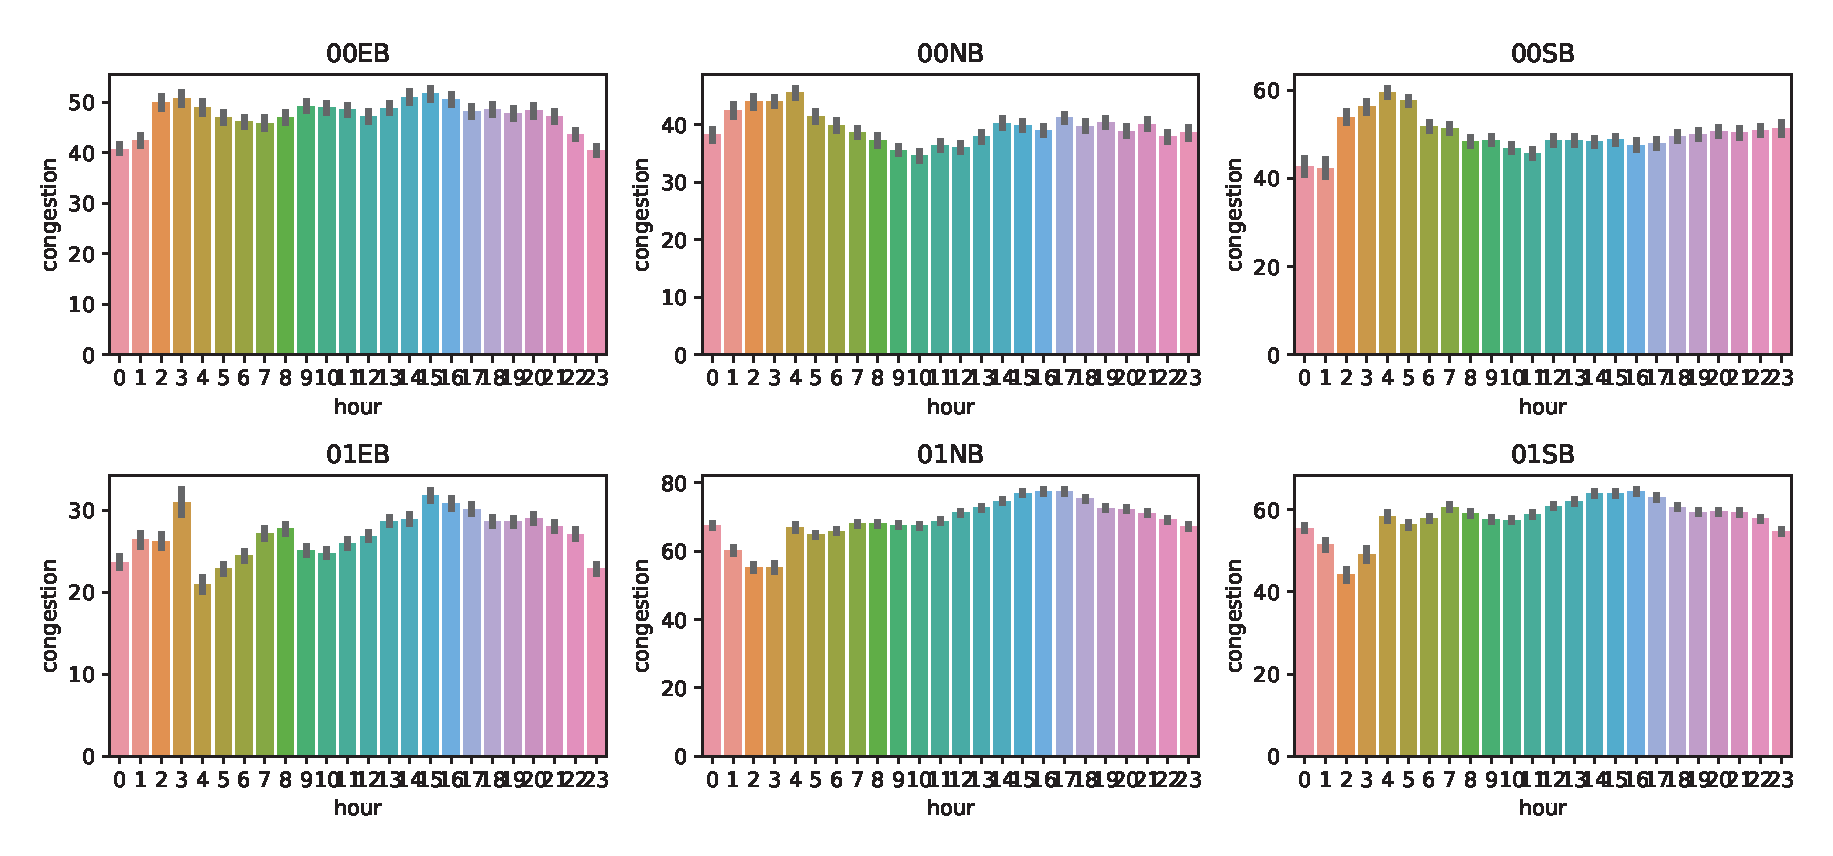
\includegraphics[scale=0.65]{figure/road.eps}
		\centering
		\caption{The effect of hour on congestion group by road}
		\label{group by road}
	\end{figure}
\end{slide}
%%
%%==========================================================================================
\begin{slide}[toc=,bm=]{The effect of weekday on congestion group by hour }
	\begin{figure}
		\setlength{\abovecaptionskip}{0.4cm} 
		\raggedleft
		\includegraphics[scale=0.35]{figure/hour.eps}
		\centering
		\caption{The effect of weekday on congestion group by hour}
		\label{group by hour}
	\end{figure}
\end{slide}
%%
%%==========================================================================================
\begin{slide}[toc=,bm=]{The effect of period on congestion}
\begin{center}
	\begin{figure}
		\setlength{\abovecaptionskip}{0.4cm} 
		\raggedleft
		\includegraphics[scale=0.45]{figure/period.eps}
		\centering
		\caption{The effect of period on congestion}
		\label{gperiod}
	\end{figure}
\end{center}
\end{slide}
%%
%%==========================================================================================
\section{ Model Train and Evaluation}


%%==========================================================================================
%%
\begin{slide}{Model Train}

\begin{center}
\begin{itemize}

\item
\smallskip
\large
{Train\\
Model: LightGBM(GPU)\\

Data: train data(fit_transform)\\

Train_test_split:x_train, x_eval, y_train, y_eval
}

\end{itemize}
\end{center}
\end{slide}
%%
%%==========================================================================================

\begin{slide}{Feature Importance}
	\begin{figure}
		\includegraphics[scale=0.9]{figure/feature_importance.eps}\\	
	\end{figure}
\end{slide}
%%
%%==========================================================================================


%%==========================================================================================
%%
\begin{slide}{Evaluation}
\begin{center}
\begin{table}[tb]
\setlength{\abovecaptionskip}{0pt}
\setlength{\belowcaptionskip}{10pt}
\centering
\caption{Model evaluation indexes}

\begin{tabular}{ c | c  }
\toprule
Index    &  Eexplication \\
\midrule
explained_variance_score     &  \makecell{Explain the variance score of \\the regression model. }   \\
mean_absolute_error		  &  \makecell{Assess the proximity of the predicted results to\\the real data set.} \\
Mean squared error				  &  \makecell{Calculate the mean value of the square sum of the errors\\ of the corresponding sample points of the \\fitting data and the original data} \\
r2_score				  			 &   \makecell{Judge the fitting degree of prediction model and real data} \\
\bottomrule
\end{tabular}
\end{table}
\end{center}
\end{slide}
%%==========================================================================================




%%==========================================================================================
%%
\begin{slide}[toc=,bm=]{Evaluation Result}
The evaluation results are as follows:

\begin{table}[tb]
\setlength{\abovecaptionskip}{10pt}
\setlength{\belowcaptionskip}{10pt}
\centering
\caption{The Evaluation results}

\begin{tabular}{p{7cm}p{4cm}}
\hline
  Index & Result  \\
\hline
  explained_variance_score   & 0.7277243544483329    \\
  mean_absolute_error&  6.167491947603395 \\
  r2_score & 0.7277251135484366  \\
\hline
\end{tabular}
\end{table}
\end{slide}
%%
%%==========================================================================================
%%==========================================================================================
%%

\section{Result}

%%==========================================================================================
%%
\begin{slide}[toc=,bm=]{Prediction Result}
	\begin{table}[tb]
		\setlength{\abovecaptionskip}{10pt}
		\setlength{\belowcaptionskip}{15pt}
		\centering
		\caption{The prediction results}
		
		\begin{tabular}{p{2.5cm}p{2.5cm}p{2.5cm}p{2.5cm}}
		\hline
		  Row_id & Congestion  &  Row_id & Congestion \\
		\hline
		848835 & 47 & 848836 & 33\\
		848837 & 39 & 848838 & 54\\
		848839 & 64 & 848840 & 23\\
		848841 & 28 & 848842 & 70\\
		848843 & 25 & 848844 & 47\\
		848845 & 46 & 848846 & 25\\
		848847 & 69 & 848848 & 60\\
		\hline
		\end{tabular}
		\end{table}
%%==========================================================================================
\end{slide}
%%
%%==========================================================================================

%%==========================================================================================
% TODO: Contact Page
\begin{wideslide}[toc=,bm=]{Contact Information}
\centering
\vspace{\stretch{1}}
\twocolumn[
lcolwidth=0.35\linewidth,
rcolwidth=0.65\linewidth
]
{
% \centerline{\includegraphics[scale=.2]{tulip-logo.eps}}
}
{
\vspace{\stretch{1}}
Associate Professor Jingbao Luo\\
School of Economics and Management\\
Nanjing University of Science and Technology, China
\begin{description}
 \item[\textcolor{orange}{\faEnvelope}] \href{mailto:jluo@tulip.org.au}
 {\textsc{\footnotesize{jluo@tulip.org.au}}}

 \item[\textcolor{orange}{\faHome}] \href{http://www.tulip.org.au}
 {\textsc{\footnotesize{Team for Universal Learning and Intelligent Processing}}}
\end{description}
}
\vspace{\stretch{1}}
\end{wideslide}

\end{document}

\endinput
